\documentclass[12pt]{article}
\usepackage{graphicx}
\usepackage{verbatim}
\begin{document}

\begin{titlepage}
\title{
Report on Analytic Solution for Annular Ducts}


\author{ Jeff Severino
 \\
University of Toledo \\
Toledo, OH  43606 \\
email: jseveri@rockets.utoledo.edu  }

\maketitle

\end{titlepage}

\section{Current Research Direction}
 The goal is to currently compute the coefficients $A$ and $B$, the weighting
 factors for the Bessel Functions for the first and second kind. V072
 contains FORTRAN subroutines that compute these along with the Bessel functions.

  
\section{Research Performed This Week}
There are four subroutines 

\begin{itemize}
    \item \verb|eigen.f|, 
        \subitem Computes the weighting factors, $A$ and $B$ for the radial mode
        shpe
    \item \verb|besj.f|, 
        \subitem Computes the bessel functions of the first kind and their derivatives
        of positive or zero order, n, and zero or positive argument x 
    \item \verb|besy.f|, and 
        \subitem Computes the bessel function of the second kind and their 
        derivatives of positive or zero order, n, and zero or positive argument x 
    \item \verb|rmode.f|. 
        \subitem Calculate radial mode shape psi for the (m,n) radial mode of an annular duct 
\end{itemize}

\section{Issues and Concerns}
After reviewing C.S. ventres,et al., "Turbofan Noise Generation", NASA-CR-167951,July 1982,
the input to  \verb|eigen.f| needed to be non-dimensional. The value of the duct mode
radial eigenvalue needs to be multiplied by the radius as directed. 
$m = 0$
$r_{min} = 0.2 $ 
$r_{max} = 1$
 $A= 1.0432423009108394$
 $B= 3.123012599045477E-02$
 $\kappa_{mn} =0.2$
 \begin{figure}
     \centering
     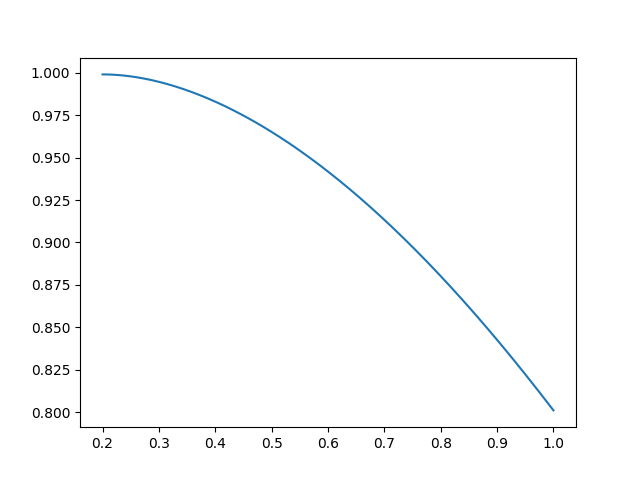
\includegraphics{Figure_1_example.png}
     \caption{Trial 1}
 \end{figure}
\section{Planned Research}
I need to comppare against a SWIRL result, however when extending $r_{max}$ to 10
the result looks pretty close to $J_0$
 \begin{figure}
     \centering
     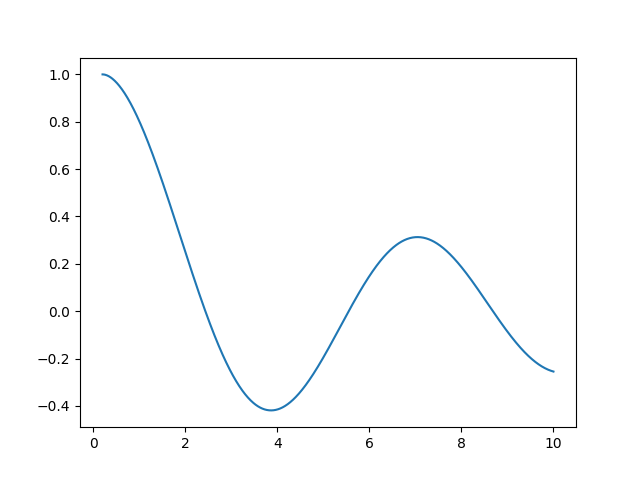
\includegraphics{Figure_1.png}
     \caption{Trial 1}
 \end{figure}
\end{document}
